%%%%%%%%%%%%%%%%%%%%%%%%%%%%%%%%%%%%%%%%%
%
% (c) 2018 by Jennifer Laaser
%
% This work is licensed under the Creative Commons Attribution-NonCommercial-ShareAlike 4.0 International License. To view a copy of this license, visit http://creativecommons.org/licenses/by-nc-sa/4.0/ or send a letter to Creative Commons, PO Box 1866, Mountain View, CA 94042, USA.
%
% The current source for these materials is accessible on Github: https://github.com/jlaaser/pogil-polymers
%
%%%%%%%%%%%%%%%%%%%%%%%%%%%%%%%%%%%%%%%%%

\documentclass[book]{pogil}

%%%%%%%%%%%%%%%%% DOCUMENT INFORMATION %%%%%%%%%%%%%%%%%%%%%%%%

\author{Jennifer Laaser}
\institution{University of Pittsburgh}
\title{POGIL Polymers}
\subtitle{Guided-Inquiry Activities \\for Polymer Chemistry and Polymer Physics}
\date{\today}

\copyrightshort{\includegraphics[width=0.1\textwidth]{by-nc-sa} J. Laaser 2018}
\copyrightfulltext{
	\textcopyright 2018 by Jennifer Laaser. Except where otherwise noted, \thetitle\ is made available under a Creative Commons Attribution-NonCommercial-ShareAlike 4.0 International License: \url{http://creativecommons.org/licenses/by-nc-sa/4.0/}

	The current source for these materials is accessible on Github:\\ 		\url{https://github.com/jlaaser/pogil-polymers}
}
\copyrightgraphic{by-nc-sa}


%%%%%%%%%%%%%%%%%%%%%%%%%%%%%%%%%%%%%%%%%%%%%%%%%%%%%%%%%%%%%%
%%%%%%%%%%%%%%%%%%%%%%%%%%%%%%%%%%%%%%%%%%%%%%%%%%%%%%%%%%%%%%

\begin{document}

\frontmatter
\pagestyle{empty}
\titlepage
\clearpage

\copyrightpage
\clearpage

\tableofcontents*
\clearpage

%\chapter{Introduction}

%\lipsum[1-12]

\mainmatter
\pagestyle{fancy}

\part{Introduction to Polymers}

	\chapter{From Molecules to Polymers}

\part{Polymer Chemistry}

	\chapter{Fundamentals of Polymer Chemistry}

	\chapter{Step-Growth Polymerizations}
		%%%%%%%%%%%%%%%%%%%%%%%%%%%%%%%%%%%%%%%%%
%
% (c) 2018 by Jennifer Laaser
%
% This work is licensed under the Creative Commons Attribution-NonCommercial-ShareAlike 4.0 International License. To view a copy of this license, visit http://creativecommons.org/licenses/by-nc-sa/4.0/ or send a letter to Creative Commons, PO Box 1866, Mountain View, CA 94042, USA.
%
% The current source for these materials is accessible on Github: https://github.com/jlaaser/pogil-polymers
%
%%%%%%%%%%%%%%%%%%%%%%%%%%%%%%%%%%%%%%%%%

\renewcommand{\figpath}{content/polymchem/stepgrowth/stepgrowth-chemistries/figs}

\begin{activity}[Condensation Polymerizations]

\begin{instructornotes}

	This activity introduces students to key chemistries used for step-growth polymerizations.
	
	After completing this activity, students will be able to:
			\begin{enumerate}
				\item Identify major classes of polymers produced by step-growth polymerization
				\item Determine the polymer produced by a given monomer or monomer pair, and determine the monomer(s) necessary to produce a target polymer
				\item Determine whether or not a reaction qualifies as a condensation polymerization, and if so, identify the small molecule released
			\end{enumerate}
	
			
	\subsection*{Activity summary:}
	\begin{itemize}
		\item \textbf{Activity type:} Learning Cycle
		\item \textbf{Content goals:} Chemistries of step-growth polymerizations
		\item \textbf{Process goals:} %https://pogil.org/uploads/attachments/cj54b5yts006cklx4hh758htf-process-skills-official-pogil-list-2015-original.pdf
			written communication, critical thinking, information processing
		\item \textbf{Duration:} TBD %approx. 45 minutes without class discussion
		\item \textbf{Instructor preparation required:} none beyond knowledge of relevant content
		\item \textbf{Related textbook chapters:}
			\begin{itemize}
				\item \emph{Polymer Chemistry} (Hiemenz \& Lodge): Table 1.2 and sections 2.2.1, 2.5, and 2.6
			\end{itemize}
	\end{itemize}

\end{instructornotes}

	%\textbf{Focus question:} Put a central question for the students to consider through this exercise here.

\begin{model}[Synthesis of a Polyester]

	Esterification reactions are a common type of reaction used to produce polymers by step-growth polymerization.
	In a typical esterification reaction, an alcohol and a carboxylic acid react to form an ester bond:
	
	\centerline{\includegraphics[width=0.7\textwidth]{\figpath/model1_ester-general.pdf}}
	
	One example of a polymerization reaction using this chemistry is the synthesis of poly(6-hydroxycaproic acid) from 6-hydroxycaproic acid monomers:
	
	\centerline{\includegraphics[width=0.9\textwidth]{\figpath/model1_P6HCA.pdf}}

\end{model}


\begin{ctqs}

	\question The 6-hydroxycaproic acid monomer is shown below: \label{ctq:label-6hcpa}
	
	\centerline{\includegraphics[width=0.3\textwidth]{\figpath/model1_6HCA.pdf}}
	
		\begin{enumerate}
			\item As drawn, what type of functional group is on the \emph{left} side of the monomer?
			
				\begin{solution}[0.5in]
					carboxylic acid (``acid'' is also fine)
				\end{solution}
			
			\item As drawn, what type of functional group is on the \emph{right} side of the monomer?
			
				\begin{solution}[0.5in]
					alcohol (or hydroxyl)
				\end{solution}
		\end{enumerate}
		
\end{ctqs}

\begin{infobox}

	When a monomer used in a step-growth polymerization has different reactive functional groups on each end, it is called an ``AB-type'' monomer.
	
	When a monomer used in a step-growth polymerization has the same reactive functional group on each end, it is called an ``AA-type'' or ``BB-type'' monomer.

\end{infobox}

\begin{ctqs}
		
		\question Would you classify the poly(6-hydroxycaproic acid) monomer used in this synthesis as an AA-type monomer or an AB-type monomer?  Briefly explain your answer in 1-2 complete sentences.
			
				\begin{solution}[1.25in]
					This is an AB-type monomer, because it has two different reactive functional groups in the same monomer.
				\end{solution}
		
		\question The synthesis of a short 6-hydroxycaproic acid oligomer from three monomers is shown explicitly, below: \label{ctq:6hcpa-oligomer}
	
\vspace{0.25in}	\centerline{\includegraphics[width=0.9\textwidth]{\figpath/model1_3oligomer-explicit.pdf}}
The molecules are color-coded so that you can see which atoms in the oligomer came from which monomer.
		
		\begin{enumerate}
		
			\item Explain, in one or two complete sentences, why you think we classify this polymer as a ``polyester'':
			
				\begin{solution}[2in]
					We call this polymer a ``polyester'' because it has ester groups in the polymer backbone.
					
					Note: the fact that they are in the backbone is important; if the ester groups are only in the sidechains, the polymer is \emph{not} a polyester.
				\end{solution}
		
			\item Explain, in one or two complete sentences, why we generally abbreviate the product of this reaction as
	
	\centerline{\includegraphics[width=0.25\textwidth]{\figpath/model1_3oligomer-shorthand.pdf}}
	
	rather than as
	
	\centerline{\includegraphics[width=0.7\textwidth]{\figpath/model1_incorrect-shorthand.pdf}}
			
				\begin{solution}[1.5in]
					We use the first notation because all of the atoms in a single repeat unit come from the same monomer (if you draw these parentheses on the color-coded molecules at the beginning of the question, each pair of parentheses will only have one color of atoms in it).  This is not true for the second and third options.
				\end{solution}
	
			\item When we write the structure of this oligomer as
	
	\centerline{\includegraphics[width=0.25\textwidth]{\figpath/model1_3oligomer-shorthand.pdf}}
	
	how many monomers make up each repeat unit in the polymer chain?
			
				\begin{solution}[0.5in]
					one
				\end{solution}
			
		\end{enumerate}
	
	\question Consider the following polymer:
	
	\centerline{\includegraphics[width=0.1\textwidth]{\figpath/model1_PMA.pdf}}
	
		\begin{enumerate}
		
			\item Would you be able to produce this polymer by esterification reactions of small molecules?  Why or why not?
			
				\begin{solution}[1.75in]
					No.  This polymer (poly(methyl acrylate)) contains ester bonds, but they are only in the sidechains, not the backbone.  But when we produce a polymer from esterification reactions of small molecules, the ester bonds end up in the polymer backbone.
					
					Put another way, the backbone in this polymer only contains carbon-carbon bonds, which cannot be formed by esterification reactions.
				\end{solution}
			
			\item Based on your answer to the previous question, would you classify this polymer as a polyester?  Why or why not?
			
				\begin{solution}[1.25in]
					No, this is not a polyester because it does not contain ester bonds in the polymer backbone.
				\end{solution}
			
		\end{enumerate}
		
\end{ctqs}
	

\begin{model}[Synthesis of a Polyamide]

Amidation reactions are another type of reaction used to produce polymers by step-growth polymerizations.
For example, acid chlorides can be reacted with primary amines to form an amide bond:
	
	\centerline{\includegraphics[width=0.7\textwidth]{\figpath/model2_amide-general.pdf}}

Commercially, this reaction is used to produce Nomex, a heat-resistant polymer used in oven mitts and firefighters' protective clothing, among other applications.
A reaction scheme for the synthesis of Nomex is shown below:
	
	\centerline{\includegraphics[width=0.9\textwidth]{\figpath/model2_Nomex.pdf}}

\end{model}

\begin{ctqs}
		\question Why is this polymer classified as a polyamide?
			
				\begin{solution}[2in]
					This polymer is classified as a polyamide because it has amide bonds in the polymer backbone.
				\end{solution}
		
		\question What functional groups does monomer 1 have?   Would you classify this monomer as an AA-type monomer or an AB-type monomer?
			
				\begin{solution}[0.75in]
					Monomer 1 has two amine groups.  Because it has two of the same reactive group, it is an AA-type monomer.
				\end{solution}
		
		\question What functional groups does monomer 2 have?   Would you classify this monomer as an AA-type monomer or an AB-type monomer?
			
				\begin{solution}[0.75in]
					Monomer 2 has two acid chloride groups.  Because it has two of the same reactive group, it is an AA-type monomer.
				\end{solution}
		
		\question Explain, in one or two complete sentences, why we might describe this reaction as an ``AA+BB''-type polymerization:
			
				\begin{solution}[1.25in]
					This polymer is formed from two AA-type monomers.  Since the two monomers are chemically different, we distinguish them by calling one the ``AA-type'' monomer and the other a ``BB-type'' monomer; thus, we call the polymerization an ``AA+BB''-type polymerization.
					
					This reaction is notably different from the AB-type polymerization in Model 1 because it requires two chemically distinct monomers; in the AB-type polymerization in Model 1, we only needed one type of monomer.
				\end{solution}
		
		\question How many monomers make up each repeat unit?
			
				\begin{solution}[0.5in]
					two
				\end{solution}
		
		\question A very similar reaction can be used to make Kevlar, the high-strength polymer used in bulletproof vests and cut-resistant gloves.  Given that Kevlar is produced from the following two monomers,
		
	
	\centerline{\includegraphics[width=0.5\textwidth]{\figpath/model2_Kevlar-monomers.pdf}}
		
		what do you predict the structure of the polymer should look like?
			
				\begin{solution}[1.5in]
					\instructordisplay{\centerline{\includegraphics[width=0.4\textwidth]{\figpath/model2_Kevlar.pdf}}}
				\end{solution}
		
		\question A similar chemistry can also be used to prepare nylon-6,6, a polymer used in many consumer goods.
		The structure of nylon-6,6 is shown below:
		
			\centerline{\includegraphics[width=0.45\textwidth]{\figpath/model2_nylon66.pdf}}
			
		What two monomers would you need to combine to make this polymer?
			
				\begin{solution}[2in]
					\instructordisplay{\centerline{\includegraphics[width=0.6\textwidth]{\figpath/model2_nylon66-monomers.pdf}}}
				\end{solution}
			
\end{ctqs}
	
\begin{infobox}

A polymerization reaction is called a \emph{condensation} polymerization if the reaction produces a small-molecule byproduct that is not part of the polymer chain.

\end{infobox}
	
\begin{ctqs}
		\question Is the esterification reaction in Model 1 a condensation polymerization?  If so, what is the small-molecule byproduct that is produced?
			
				\begin{solution}[1in]
					Yes, the reaction in Model 1 is a condensation polymerization. It produces \ce{H2O}.
				\end{solution}
		
		\question Is the amidation reaction in Model 2 a condensation polymerization?  If so, what is the small-molecule byproduct that is produced?
			
				\begin{solution}[1in]
					Yes, the reaction in Model 2 is a condensation polymerization. It produces \ce{HCl}.
				\end{solution}
		
\end{ctqs}

\begin{model}[Other Chemistries used for Step-Growth Polymerization]

Shown below are reactions used to produce a variety of other commercially-important polymers by step-growth polymerization:

\vspace{0.1in}

\textbf{a) polycarbonate} (high transparency and impact resistance; used in DVDs, glasses, etc.)
		
			\centerline{\includegraphics[width=\textwidth]{\figpath/model3_polycarbonate.pdf}}

\vspace{0.1in}

\textbf{b) polyurethanes} (foams; thermoplastic elastomers, e.g. spandex)
		
			\centerline{\includegraphics[width=\textwidth]{\figpath/model3_polyurethane.pdf}}

\vspace{0.1in}

\textbf{c) epoxies} (adhesives; coatings)
		
			\centerline{\includegraphics[width=\textwidth]{\figpath/model3_epoxy.pdf}}

\end{model}

\vspace{0.25in}
\begin{ctqs}

		\question Classify each of the reactions in the above Model as either an ``AB-type'' or ``AA+BB-type'' polymerization:
		
			\begin{enumerate}
				\item ~ \begin{solution}[0.6in]AA+BB-type\end{solution}
				\item ~ \begin{solution}[0.6in]AA+BB-type\end{solution}
				\item ~ \begin{solution}[0.6in]AA+BB-type\end{solution}
			\end{enumerate}
			
		% may need another question in here
		
		\clearpage
		\question Complete the following table for the polymerizations depicted in Models 1-3:
		
			\begin{center}
				\begin{tabular}{|c|c|c|c|c|}
				\hline
					Polymer & ``A'' reactive group & ``B'' reactive group & ``ab'' bond formed & \begin{tabular}{c}Small\\ Molecule\\Byproduct\end{tabular} \\\hline
					Polyester &						
						\includegraphics[width=0.12\textwidth]{\figpath/model3_hydroxyl.pdf} &
						\includegraphics[width=0.15\textwidth]{\figpath/model3_acid.pdf} &
						\includegraphics[width=0.15\textwidth]{\figpath/model3_ester.pdf}&
						\answer{\includegraphics[width=0.08\textwidth]{\figpath/model3_H2O-red.pdf}}\\\hline
					Polyamide &
						\includegraphics[width=0.12\textwidth]{\figpath/model3_amine.pdf} &
						\includegraphics[width=0.15\textwidth]{\figpath/model3_acidchloride.pdf} &
						\answer{\includegraphics[width=0.15\textwidth]{\figpath/model3_amide-red.pdf}}&
						\includegraphics[width=0.08\textwidth]{\figpath/model3_HCl.pdf} \\\hline
					Polycarbonate &
						
\includegraphics[width=0.004\textwidth]{\figpath/model3_blank.pdf}\answer{\includegraphics[width=0.12\textwidth]{\figpath/model3_hydroxyl-red-right.pdf}}&
						\answer{\includegraphics[width=0.15\textwidth]{\figpath/model3_phosgene-red.pdf}}&
						\answer{\includegraphics[width=0.15\textwidth]{\figpath/model3_carbonate-red.pdf}}& 
						\answer{\includegraphics[width=0.08\textwidth]{\figpath/model3_HCl-red.pdf}}\\\hline
					Polyurethane &
						
\includegraphics[width=0.004\textwidth]{\figpath/model3_blank.pdf}\answer{\includegraphics[width=0.12\textwidth]{\figpath/model3_isocyanate-red.pdf}}&
						\answer{\includegraphics[width=0.12\textwidth]{\figpath/model3_hydroxyl-red-left.pdf}}& 
						\answer{\includegraphics[width=0.15\textwidth]{\figpath/model3_urethane-red.pdf}}&
						\answer{\includegraphics[width=0.08\textwidth]{\figpath/model3_HCl-red.pdf}}\\\hline
					Epoxy &
						
\includegraphics[width=0.004\textwidth]{\figpath/model3_blank.pdf}\answer{\includegraphics[width=0.12\textwidth]{\figpath/model3_amine-red.pdf}}&
						\answer{\includegraphics[width=0.12\textwidth]{\figpath/model3_epoxide-red.pdf}}&
						\answer{\includegraphics[width=0.15\textwidth]{\figpath/model3_epoxy-red.pdf}}&
						\answer{none} \\\hline
				\end{tabular}
			\end{center}
			
		\vspace{0.25in}
		\question Which of the above polymerization reactions would you classify as condensation polymerizations?
			
				\begin{solution}[2in]
					All of the reactions except for the epoxy reaction form a small-molecule byproduct, so all of the reactions except for the epoxy reaction are condensation polymerizations.
				\end{solution}
			
\end{ctqs}
	

\clearpage
\begin{exercises}

		\exercise (other esterification chemistries)
		
		\exercise (difference in polymer structures formed by AB vs AA+BB reactions?)
		
		\exercise (H-bonded structure of polyesters vs. polyamides - justify difference in properties?)
		
		\exercise (phosgene alternatives for polycarbonate synthesis?)
		
		\exercise (epoxidation reaction formed a linear polymer with secondary amines.  however, secondary amines can also attack epoxides.  What type of polymer structure would be formed in this case?)
		
\end{exercises}
	
\end{activity}
		%%%%%%%%%%%%%%%%%%%%%%%%%%%%%%%%%%%%%%%%%
%
% (c) 2018 by Jennifer Laaser
%
% This work is licensed under the Creative Commons Attribution-NonCommercial-ShareAlike 4.0 International License. To view a copy of this license, visit http://creativecommons.org/licenses/by-nc-sa/4.0/ or send a letter to Creative Commons, PO Box 1866, Mountain View, CA 94042, USA.
%
% The current source for these materials is accessible on Github: https://github.com/jlaaser/pogil-polymers
%
%%%%%%%%%%%%%%%%%%%%%%%%%%%%%%%%%%%%%%%%%

\renewcommand{\figpath}{content/polymchem/stepgrowth/Mn-and-stoich/figs}

\begin{activity}[Degree of Polymerization in Step-Growth Polymerizations]

	%\textbf{Focus question:} Put a central question for the students to consider through this exercise here.

\begin{model}[Polymerization of ``AB''-Type Monomers]

The simplest type of step-growth polymerization is one in which each monomer has one ``A''-type reactive group and one ``B''-type reactive group.
These types of monomers are referred to as ``AB''-type monomers.

In each step of the polymerization, an ``A'' group on one molecule reacts with a ``B'' group on another molecule to form an ``ab'' bond, as shown below:

\vspace{0.1in}
\centerline{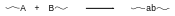
\includegraphics[width=0.6\textwidth]{\figpath/ABrxn.pdf}}

For example, for a simple reaction mixture containing 8 ``AB''-type monomers, the evolution of the reaction mixture might look something like this:

\vspace{0.1in}
\centerline{\includegraphics[width=0.9\textwidth]{\figpath/ABpolym.pdf}}

\end{model}

\begin{ctqs}

	\question \label{ctq:ABtable} For the reaction mixture shown in Model 1, fill out the following table:
		
			\begin{table}[h]
				\centering
				\renewcommand{\arraystretch}{3}
				\begin{tabular}{|c|c|c|}
					\hline
					\textbf{Step} &  \textbf{Number of unreacted ``A'' groups} & \textbf{Number of molecules} \\\hline
					0 && \\\hline
					1 && \\\hline
					2 && \\\hline
					3 && \\\hline
					4 && \\\hline
				\end{tabular}
			\end{table}
		
	\question Explain, in a complete sentence, how the number of molecules in the mixture is related to the number of unreacted ``A'' groups.
		
		\vspace{1in}
		
		\question The number-average degree of polymerization, $N_n$, is the total number of \emph{monomers} divided by the total number of \emph{molecules}.  Remembering that we started with 8 monomers, calculate the number-average degree of polymerization for each step shown in Model 1.
		
			\begin{table}[h]
				\centering
				\renewcommand{\arraystretch}{3}
				\begin{tabular}{|c|c|c|c|c|c|}
					\hline
					\textbf{~~Step~~} &  \textbf{~~~~0~~~~} & \textbf{~~~~1~~~~} & \textbf{~~~~2~~~~} & \textbf{~~~~3~~~~} & \textbf{~~~~4~~~~} \\\hline
					$\mathbf{N_n}$ &&&&& \\\hline
				\end{tabular}
			\end{table}
		
		\question Suppose that you had initially started with 100 monomers.  Then, suppose that at some time later, you had only 8 unreacted ``A'' groups left.
		
			\begin{enumerate}
				\item How many molecules would there be in the reaction mixture at this point?
				
				\item What would the number-average degree of polymerization be at this point?
			\end{enumerate}
			
		\question More generally, suppose you started with $v_A^0$ monomers, and at some time later, you had only $v_A$ unreacted ``A'' groups left.  What would the number average-degree of polymerization be at this point, in terms of $v_A^0$ and $v_A$?
		
		\vspace{1in}
		
\end{ctqs}
	
\begin{infobox}

Usually, we find it more useful to work in terms of the \emph{fraction} of all ``A'' groups that have reacted, rather than the total \emph{number} of ``A'' groups that have reacted.  In step-growth polymerizations, we refer to the fraction of ``A'' groups that have reacted as the ``extent of reaction'', $p$.

\end{infobox}
	
\begin{ctqs}
		\question If we start with $v_A^0$ ``A'' groups, how many of the ``A'' groups will have \emph{reacted} when the extent of reaction is equal to $p$?
		
		\vspace{1in}
		
		\question How many ``A'' groups are still \emph{unreacted} when the extent of reaction is equal to $p$?
		
		\vspace{1in}
		
		\question Using your answers to critical thinking questions 5, 6, and 7, derive an expression for $N_n$ in terms of $p$.
		
		\vspace{1in}
		
\end{ctqs}

\begin{model}[Polymerization of ``AA'' and ``BB''-Type Monomers]

Now, let's consider a slightly more complicated reaction, with two different types of monomers that each have \emph{either} two ``A'' reactive groups \emph{or} two ``B'' type reactive groups.
We call monomers with two ``A'' groups ``AA''-type monomers, and we call monomers with two ``B'' groups ``BB''-type monomers.

Suppose we start with 4 ``AA''-type monomers and 4 ``BB''-type monomers.
In this case, the evolution of the reaction mixture might look something like this:

\vspace{0.1in}
\centerline{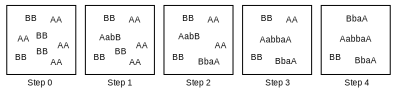
\includegraphics[width=0.9\textwidth]{\figpath/AABBpolym.pdf}}

\end{model}

\begin{ctqs}
		\question \label{ctq:AABBtable} For the reaction mixture shown in Model 2, fill out the following table:
		
			\begin{table}[!h]
				\centering
				\renewcommand{\arraystretch}{3}
				\begin{tabular}{|c|c|c|c|}
					\hline
					\textbf{Step} &  \textbf{Number of unreacted ``A'' groups} & \textbf{Number of molecules} & ~~~~$\mathbf{N_n}$~~~~\\\hline
					0 &&& \\\hline
					1 &&& \\\hline
					2 &&& \\\hline
					3 &&& \\\hline
					4 &&& \\\hline
				\end{tabular}
			\end{table}
			
		\question Compare your answers in question \ref{ctq:AABBtable} with those from question \ref{ctq:ABtable}.  What similarities and/or differences do you notice?
		
		\vspace{1in}
		
		\question Consider the following statement:
		
			\emph{``In polymerizations of AA- and BB-type monomers, we should be able to use the same expressions to calculate $N_n$ as we did for polymerizations of AB-type monomers.''}
			
			In two or three complete sentences, briefly critique or defend this statement, making sure to explain your reasoning.
		
		\vspace{1.5in}
			
\end{ctqs}
	
\begin{infobox}

A reaction is \emph{stoichiometrically balanced} if the initial reaction mixture contains exactly the same number of ``A'' and ``B'' reactive groups.

\end{infobox}
	
\begin{ctqs}
		\question Are the reactions in Models 1 and 2 stoichiometrically balanced?  Briefly explain your answer in one or two complete sentences.
		
		\vspace{1in}
		
		\question Predict what the reaction mixtures in Models 1 and 2 might look like if you let them react until no more reactions could take place:
		
\vspace{0.1in}
\centerline{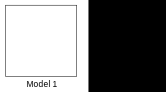
\includegraphics[width=0.75\textwidth]{\figpath/Model1and2_blank.pdf}}
		
		\question Calculate the number-average degree of polymerization for both of the ``final'' states you drew in response to the previous question:
		
		\vspace{1in}
\end{ctqs}

\begin{model}[A Stoichiometrically-Imbalanced Reaction Mixture]

Practically speaking, it is often very difficult to ensure that a reaction mixture is perfectly stoichiometrically-balanced, and there is often a small excess of one type of monomer or the other.

Consider a reaction mixture that starts with 3 AA-type monomers and 5 BB-type monomers:

\vspace{0.1in}
\centerline{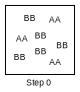
\includegraphics[width=0.9\textwidth]{\figpath/AABBpolym-nonstoich.pdf}}

\end{model}

\begin{ctqs}

		\question Fill in the blank spaces in the model, above, with reasonable predictions for what the reaction mixture might look like in each successive step.
		
		\question Which type of reactive group is the ``limiting reagent'' in this reaction?
		
		\question \label{ctq:nonstoichpredict} Predict what the reaction mixture in Model 3 might look like if you let it react until no more reactions could take place:
		
\vspace{0.1in}
\centerline{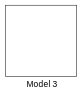
\includegraphics[width=0.3\textwidth]{\figpath/Model3_blank.pdf}}
		
		\question Calculate the number-average degree of polymerization for the ``final'' state you drew in response to the previous question:
		
		\vspace{1in}
		
		\question Is the final degree of polymerization for this stoichiometrically-unbalanced reaction smaller than, equal to, or larger than the final degree of polymerization you calculated for the stoichiometrically-balanced reactions in Models 1 and 2?
		
		\vspace{0.5in}
		
		\question Which type of reactive group is on the ends of all of the chains you drew in question \ref{ctq:nonstoichpredict}?
		
		\vspace{0.5in}
		
		\question Briefly critique or defend the following statement:
		
			\emph{``When drawing the structure of a polymer produced by a step-growth polymerization, we should always make sure that we draw end groups consistent with whichever reactive species was present in excess.''}
		
		\vspace{1in}
			
\end{ctqs}
	
\begin{infobox}

In stoichiometrically-imbalanced step-growth polymerizations with an excess of B groups, we define a parameter $r$ that reflects the ratio of A groups to B groups.	
	If the initial number of A groups is $v_A^0$ and the initial number of B groups is $v_b^0$, then
	\begin{equation*}
		r = \frac{v_A^0}{v_B^0}
	\end{equation*}
	
	
	For a reaction mixture with stoichiometric imbalance $r$ at extent of reaction $p$, the number-average degree of polymerization is given by
	\begin{equation*}
		N_n = \frac{1+r}{1+r-2pr}
	\end{equation*}
	
\end{infobox}
	
\begin{ctqs}
		%\question When $r=1$, how can you simplify this expression for $N_n$?		
		%\question When $p=1$, how can you simplify this expression for $N_n$?
		\question Using this expression, fill in the following table with the expected number-average degree of polymerization for different combinations of $r$ and $p$ values:
		
			\begin{table}[!h]
				\centering
				\renewcommand{\arraystretch}{3}
				\begin{tabular}{|c|c|c|c|}
					\hline
					 &  ~$p=0.9$~ & ~$p=0.99$~ & ~$p=0.999$~ \\\hline
					$r=0.9$ &&& \\\hline
					$r=0.99$ &&& \\\hline
					$r=0.999$ &&& \\\hline
				\end{tabular}
			\end{table}
		
		\question On the basis of your answers to the previous question, briefly critique or defend the following statement:
		
			\emph{``Achieving high molecular weights in step-growth polymerizations requires both very precise measurement of the reagents, and reaction conditions which strongly favor the bond-forming reaction.''}
			
\end{ctqs}

\begin{exercises}
	
		\exercise In this activity, we only calculated the number-average \emph{degree of polymerization} of the polymers produced in step-growth polymerizations. However, usually, we want to be able to calculate the \emph{molecular weight} of the polymers as well.
		
			\begin{enumerate}
				\item In Model 1, we considered a reaction of AB-type monomers.  If each monomer had mass $m_{AB}$, how would you calculate the number-average molecular weight, $M_n$, of the polymer produced when the extent of reaction is equal to $p$?
				
				\item In Model 2, we considered a stoichiometrically-balanced reaction of AA- and BB-type monomers. If the AA-type monomers each had mass $m_{AA}$ and the BB-type monomers each had mass $m_{BB}$, how would you calculate the number-average molecular weight of the polymer produced when the extent of reaction is equal to $p$?
				
					\emph{Note: this question is a little tricky - remember that $N_n$ counts \emph{monomers}, but in this reaction, not all of the monomers have the same molecular weight.  How might you be able to correct for this?}
				
			\end{enumerate}
		
		\exercise In Model 3, we considered a stoichiometrically-imbalanced reaction of AA- and BB-type monomers.  However, another important limit occurs when we have equal numbers of AA- and BB-type monomers, but add in an extra monofunctional reagent ``Bx'' that can only react on one side.
		
			\begin{enumerate}
				\item How many ``Bx'' molecules would you need to add to the reaction mixture to have the same number of extra ``B'' groups as you would get from a single extra BB-type monomer?
				
				\item (Modify stoich imbalance eqn to reflect this case?)
				
				\item Monofunctional reagents are a common impurity in supplies of difunctional monomers. Briefly explain why this means it is necessary to rigorously purify the starting materials used in step-growth polymerizations.
			\end{enumerate}
\end{exercises}
	
\end{activity}
		%%%%%%%%%%%%%%%%%%%%%%%%%%%%%%%%%%%%%%%%%
%
% (c) 2018 by Jennifer Laaser
%
% This work is licensed under the Creative Commons Attribution-NonCommercial-ShareAlike 4.0 International License. To view a copy of this license, visit http://creativecommons.org/licenses/by-nc-sa/4.0/ or send a letter to Creative Commons, PO Box 1866, Mountain View, CA 94042, USA.
%
% The current source for these materials is accessible on Github: https://github.com/jlaaser/pogil-polymers
%
%%%%%%%%%%%%%%%%%%%%%%%%%%%%%%%%%%%%%%%%%

\renewcommand{\figpath}{content/polymchem/stepgrowth/dispersity/figs}

\begin{activity}[Molecular Weight Distributions in Step-Growth Polymerizations]

\begin{instructornotes}

	This activity introduces students to key concepts related to the molecular weight distributions obtained in step-growth polymerizations.
	
	After completing this activity, students will be able to:
			\begin{enumerate}
				\item Calculate the fraction of polymer chains with length $i$ in a step-growth polymerization,
				\item Describe, qualitatively, the chain length distribution and how it changes with extent of reaction,
				\item Calculate the expected dispersity for step-growth polymerizations, and
				\item Explain why the limiting dispersity for a step-growth polymerization is 2.
			\end{enumerate}
			
	\subsection*{Activity summary:}
	\begin{itemize}
		\item \textbf{Activity type:} Learning Cycle
		\item \textbf{Content goals:} Molecular weight distributions and dispersity in step-growth polymerizations
		\item \textbf{Process goals:} %https://pogil.org/uploads/attachments/cj54b5yts006cklx4hh758htf-process-skills-official-pogil-list-2015-original.pdf
			written communication, critical thinking, information processing
		\item \textbf{Duration:} 25-30 minutes, including time for discussion
		\item \textbf{Instructor preparation required:} none beyond knowledge of relevant content
		\item \textbf{Related textbook chapters:}
			\begin{itemize}
				\item \emph{Polymer Chemistry} (Hiemenz \& Lodge): section 2.4
			\end{itemize}
		\item \textbf{Facilitation notes:}
			\begin{itemize}
				\item The process described in Model 1 depicts step-growth polymerizations as a monomer-by-monomer addition process.  Although this simplification was necessary to make the model accessible to students, it is not strictly accurate, since oligomers can react with each other in step-growth polymerizations (and not just with monomers).
			\end{itemize}
	\end{itemize}

\end{instructornotes}

	%\textbf{Focus question:} Put a central question for the students to consider through this exercise here.

\begin{model}[Probabilities of Forming Different Chain Lengths]

To determine the \emph{distribution} of chain lengths formed in a step-growth polymerization, it is useful to calculate the probability of forming each different chain length.

The following diagram summarizes the steps that lead to different chain lengths in a step-growth polymerization of AB-type monomers at extent of reaction $p$:

\vspace{0.1in}
\centerline{\includegraphics[width=0.9\textwidth]{\figpath/model1-fulltree}}

In this diagram, the different \textbf{states} of the polymer chain are written in bold text.  They are connected by arrows describing the \textbf{processes} that take the chain from one state to the next; the text \emph{above} each arrow describes which process takes place, while the expression \emph{under} each arrow gives the probability of that process occurring.

\end{model}

\vspace{0.05in}
\begin{ctqs}
	
	\question What is the probability that...
	
		\begin{enumerate}
			\item ... an AB monomer does not react, and remains an AB monomer?
	
			\begin{solution}[0.25in]
				$1-p$
			\end{solution}

		\item ... an AB monomer reacts to form an AbaB dimer?
	
			\begin{solution}[0.25in]
				$p$
			\end{solution}
		
		\item ... an AbaB dimer does not react, and remains an AbaB dimer?
	
			\begin{solution}[0.25in]
				$1-p$
			\end{solution}
	
		
		\item ... an AbaB dimer reacts to form an AbabaB trimer?
	
			\begin{solution}[0.25in]
				$p$
			\end{solution}
			
		\end{enumerate}	
		
	\question For \emph{any} molecule with $n$ monomers, what is the probability that it reacts to form a molecule with $n+1$ monomers?
	
			\begin{solution}[0.25in]
				$p$
			\end{solution}
	
	\question Is your answer to the previous question consistent with the definition of the extent of reaction $p$?  Briefly explain your answer in 1-2 complete sentences.
	
		\begin{solution}[2in]
			Yes, it is.  The extent of reaction, $p$, is the fraction of ``A'' groups that have reacted.  Since each molecule has exactly 1 ``A'' group, the fraction of molecules that reach length $n$ whose ``A'' groups react to form chains with $n+1$ monomers is $p$.  This fraction is equivalent to the probability that the chain grows from $n$ to $n+1$ monomers.
		\end{solution}
	
\end{ctqs}

\begin{infobox}

	For a process with a \textbf{single} step, the overall probability of reaching the final state is just the probability of that step.
	
	For example, the series of steps that leads to a chain with exactly one monomer (i.e. an AB monomer that does not react) is shown below:
	
	\vspace{0.1in}
	\centerline{\includegraphics[width=0.3\textwidth]{\figpath/model1-AB}}
	
	Since there is only a single step in this process, the overall probability of obtaining a chain with exactly 1 monomer is just the probability of this step, or $1-p$.
	
	\vspace{0.1in}
	For processes with \textbf{multiple} steps, the overall probability of reaching the final state is the \emph{product} of the probabilities for each step in the process.
	
	For example, the series of steps takes us from an initial AB monomer to an AbaB chain that does not react further (remains a chain with exactly 2 monomers) is:
	
	\vspace{0.1in}
	\centerline{\includegraphics[width=0.6\textwidth]{\figpath/model1-AbaB}}
	
	The first step occurs with probability $p$, while the second step occurs with probability $1-p$; the total probability of obtaining a chain with exactly 2 monomers is the product of these probabilities, or $p(1-p)$.
	
\end{infobox}

\begin{ctqs}

	\question Diagram the series of steps that lead to formation of a chain with 3 monomers that does not react any further:
	
		\begin{solution}[1in]\instructordisplay{
			\centerline{ \includegraphics[width=0.8\textwidth]{\figpath/model1-AbabaB-answer}}
		}\end{solution}
	
	\question Based on your diagram, what is the overall probability of obtaining a chain with exactly 3 monomers?
	
		\begin{solution}[1in]
			$p \cdot p \cdot (1-p) = p^2(1-p)$
		\end{solution}
	
	\question Building on this process, fill in the blanks in the following table:
	
		\begin{center}
			\renewcommand{\arraystretch}{3}
			\begin{tabular}{|c|c|}
				\hline
				\textbf{~~i~~} & {\renewcommand{\arraystretch}{1}\begin{tabular}{c}\textbf{Probability that a molecule is composed}\\\textbf{of exactly $i$ monomers}\end{tabular} }\\\hline
				1 & $1-p$\\\hline
				2 & $p(1-p)$\\\hline
				3 & \answer{$p^2(1-p)$}\\\hline
				4 & \answer{$p^3(1-p)$}\\\hline
				5 & \answer{$p^4(1-p)$}\\\hline
			\end{tabular}
		\end{center}
	
	\question What pattern do you notice in these values?  Briefly describe your observations in 1-2 complete sentences.
	
		\begin{solution}[1in]
		
			The values acquire an additional factor of $p$ for each additional monomer in the chain.
		
		\end{solution}
	
	\question Complete the following statement:
	
		``The probability that a molecule is composed of exactly $i$ monomers is \line(1,0){50}.''
	
		\begin{solution}[0.5in]
		
			$p^{i-1}(1-p)$
			
		\end{solution}
		
\end{ctqs}

\begin{infobox}
	The \emph{probability} that a molecule is composed of exactly $i$ monomers is the same as the \emph{fraction of molecules} that are composed of exactly $i$ monomers.
\end{infobox}


\begin{ctqs}
	
	\question Complete the following statement:
	
		``The fraction of molecules, $x_i$, that are composed of exactly $i$ monomers is \line(1,0){50}.''
	
		\begin{solution}[0.5in]
		
			$x_i = p^{i-1}(1-p)$
			
		\end{solution}
	
	\question Using this expression, calculate the fraction of molecules that have exactly length $i$ for both $p=0.5$ and $p=0.9$ at the following values of $i$:
	
		\begin{center}
			\renewcommand{\arraystretch}{3}
			\begin{tabular}{|c|c|c|}
				\hline
				\textbf{~~$i$~~} & ~~~$x_i$ when $p=0.5$~~~ & ~~~$x_i$ when $p=0.9$~~~ \\\hline
				1 & \answer{0.5} & \answer{0.1} \\\hline
				2 & \answer{0.25} & \answer{0.09} \\\hline
				3 & \answer{0.125} & \answer{0.08} \\\hline
				5 & \answer{0.0313} & \answer{0.065} \\\hline
				10 & \answer{9.7x10$^{-4}$} & \answer{0.0387} \\\hline
				15 & \answer{3.1x10$^{-5}$} & \answer{0.0229} \\\hline
				20 & \answer{9.5x10$^{-7}$} & \answer{0.0135} \\\hline
			\end{tabular}
		\end{center}
		
		\clearpage
	\question Plot your results on the following axes.  Make sure to use a different symbol for points corresponding to $p=0.5$ than for the points corresponding to $p=0.9$.
	
		\begin{solution}[2.75in]
			\studentdisplay{
				\centerline{\includegraphics[width=0.7\textwidth]{\figpath/model1-xi-axes.pdf}}
			}
			\instructordisplay{
				\centerline{\includegraphics[width=0.7\textwidth]{\figpath/model1-xi-plotted.pdf}}
			}
		\end{solution}
	
	\question How are the plots for $p=0.5$ and $p=0.9$ similar, and how are they different?  Briefly describe your observations in 2-3 complete sentences.
	
		\begin{solution}[1.5in]
		
			Both of these plots decrease exponentially toward zero with increasing values of $i$.  However, the plot for $p=0.5$ decreases much faster, and a higher fraction of the molecules have very short chain lengths, than in the case where $p=0.9$.
		\end{solution}
	
	\question What is the \emph{most probable} chain length for each value of $p$?
	
		\begin{solution}[0.5in]
		
			The most probable chain length is just the one with the highest value of $x_i$.  Thus, the most probably chain length is $i=1$ for both values of $p$.
		
		\end{solution}
	
	\question Can the fraction of chains with length $i+1$ ever be \emph{greater} than the fraction of chains with length $i$?  Justify your answer in 1-2 complete sentences.
	
		\begin{solution}[1.5in]
		
			No, the fraction of chains with length $i+1$ can never be greater than the mole fraction of chains with length $i$.  This is because for each additional monomer, we pick up another factor of $p$; since $p$ is always less than one, $x_{i+1}$ will always be less than $x_i$.
			
			In mathematical terms, $x_i$ decreases monotonically with increasing chain length $i$.
		
		\end{solution}
	
\end{ctqs}


\begin{model}[$M_n$ and $M_w$ for Step-Growth Polymerizations]

	To calculate $M_n$ and $M_w$, we need to know $n_i$, or the total number of chains with $i$ monomers.
	
	If we started with $v_A^0$ monomers, then when the extent of reaction is equal to $p$, there will be $(1-p)v_A^0$ unreacted A groups left.  Recalling that the number of unreacted A groups is equal to the number of molecules in the reaction mixture, this lets us write
	\begin{align*}
		n_i = \text{(fraction of molecules that }&\text{have length }i\text{) x (number of molecules in reaction mixture)}\\
			%&= (x_i)((1-p)v_A^0)\\
			&= \left(p^{i-1}(1-p)\right)\left((1-p)v_A^0\right)\\
			&= p^{i-1}(1-p)^2v_A^0
	\end{align*}
	
	If we plug this expression into our equation for $M_n$, we get
	\begin{equation*}
		M_n = \frac{\sum_i n_i M_i}{\sum_i n_i} %= \frac{\sum_i p^{i-1}(1-p)^2 v_A^0 i M_0}{\sum_i p^{i-1}(1-p)^2 v_A^0} 
		= M_0\frac{\sum_i p^{i-1}(1-p)^2 i }{\sum_i p^{i-1}(1-p)^2}
	\end{equation*}
	where $M_0$ is the molecular weight of the monomer ($M_i = M_0 i$).
	
	\vspace{0.25in}
	
	If we evaluate these sums, we obtain
	\begin{align*}
		M_n = \frac{M_0}{1-p} && \text{or} && N_n = \frac{M_n}{M_0} = \frac{1}{1-p}
	\end{align*}
	which is exactly what we expected (whew - our math worked!).
	
	\vspace{0.25in}
	Similarly, if we plug this expression into our equation for $M_w$ and work through the sums, we get
	\begin{align*}
		M_w = \frac{\sum_i n_i M_i^2}{\sum_i n_i M_i} = M_0\frac{1+p}{1-p} && \text{or} && N_w = \frac{M_w}{M_0} = \frac{1+p}{1-p}
	\end{align*}

\end{model}

\begin{ctqs}
		\question Calculate the dispersity for a step-growth reaction with extent of reaction $p$.
		
			\begin{solution}[1.95in]
			
				\begin{equation*}
					\text{\DJ} = \frac{M_w}{M_n} = \frac{M_0\frac{1+p}{1-p}}{M_0\frac{1}{1-p}} = 1+p
				\end{equation*}
			\end{solution}
			
			
		\question What is the value of the dispersity when $p=0$?  Briefly comment on whether or not this answer makes sense.
		
			\begin{solution}[1.5in]
			
				When $p=0$, $\text{\DJ}=1+0 = 1$.  This does make sense: when the extent of reaction is zero, no reactions have taken place, and the reaction mixture contains only monomers.  Since all of the molecules in the mixture are thus identcail (and exactly the same size), the dispersity is 1 - the mixture is monodisperse.
			
			\end{solution}
			
			
		\question What is the value of the dispersity when $p=1$?
		
			\begin{solution}[1in]
			
				When $p=1$, $\text{DJ}=1+1=2$.  This is an important limit: the limiting dispersity for a step-growth polymerization is 2.
			
			\end{solution}
			
			
			
		\question Can the dispersity of a polymer produced by step-growth polymerization ever be greater than 2?  Briefly defend your answer in 1-2 complete sentences.
		
			\begin{solution}[1.5in]
			
				Following the argument presented in this exercise, no, the dispersity of a polymer produced by step-growth polymerization can never be greater than 2, because $p$ can never be greater than 1. 
				
				Note for instructors: practically speaking, there are certain conditions that can generate dispersities greater than 2 (for example, when the reaction mixture contains multifunctional monomers that induce chain branching, or when the monomers are added in several batches - see DOI:10.1016/0032-3861(92)90340-3), but for the purposes of this activity, students should learn that the ideal limiting dispersity for step-growth polymerizations is two.
			
			\end{solution}
			
			
\end{ctqs}

\begin{exercises}

		\exercise Suppose you synthesized a polymer by step-growth polymerization and found that it had a dispersity of 1.86.
		
			\begin{enumerate}
				\item What must the extent of reaction have been in this polymerization?
		
					\begin{solution}
					\instructordisplay{
						\begin{equation*}
							p = \text{\DJ}-1 = 1.86-1 = 0.86
						\end{equation*}
					}
					\end{solution}
					
				\item What would you expect the number-average degree of polymerization of this polymer to be?
		
					\begin{solution}
					\instructordisplay{
						\begin{equation*}
							N_n = \frac{1}{1-p} = \frac{1}{1-0.86} = 7.1
						\end{equation*}
					}
					\end{solution}
			\end{enumerate}
			
		\exercise Show that the summation expression for $M_n$ given in Model 2 simplifies to the expected result by doing the following:
		
			\begin{enumerate}
				\item First, show that the summation expression for $M_n$ given in Model 2 can be rewritten
					\begin{equation*}
						M_n = M_0 \frac{{\sum_i i p^{i-1}}}{\frac{1}{p}\sum_i p^i}
					\end{equation*}
					
					\begin{solution}\instructordisplay{
						In Model 2, $M_n$ was written as
						\begin{equation*}
							M_n = M_0\frac{\sum_i p^{i-1}(1-p)^2 i }{\sum_i p^{i-1}(1-p)^2}
						\end{equation*}
						We can simplify this by realizing that any multiplicative terms that do not depend on $i$ can be pulled out of the sum:
						\begin{equation*}
							M_n = M_0\frac{(1-p)^2\sum_i p^{i-1} i }{(1-p)^2\sum_i p^{i-1}} = M_0\frac{\sum_i p^{i-1} i }{\sum_i p^{i-1}}
						\end{equation*}
						Similarly, using $p^{i-1} = p^i/p$,
						\begin{equation*}
							M_n = M_0\frac{\sum_i p^{i-1} i }{\sum_i p^{i-1}} = M_0\frac{\sum_i p^{i-1} i }{\frac{1}{p}\sum_i p^{i}}
						\end{equation*}
						
					}\end{solution}
					
				\item The denominator of this expression is just a geometric series.  Recall that if $p < 1$, then 
		
			\begin{equation*}
				\sum_{i=1}^{\infty} p^i = \frac{p}{1-p}
			\end{equation*}
			
					Substitute this expression into your equation for $M_n$ and simplify.
					
					\begin{solution}\instructordisplay{
						\begin{align*}
							M_n &= M_0\frac{\sum_i p^{i-1} i }{\frac{1}{p}\sum_i p^{i}}\\
								&= M_0\frac{\sum_i p^{i-1} i }{\frac{1}{p}\frac{p}{1-p}}\\
								&= M_0 (1-p)\sum_i p^{i-1} i 
						\end{align*}
						
					}\end{solution}
			
				\item The remaining sum can be calculated by differentiating both sides of the equation for $\sum_i p^i$.  Carry out this differentiation to show that
						\begin{equation*}
							\sum_{i=1}^{\infty} ip^{i-1} = \frac{1}{(1-p)^2}
						\end{equation*}
				
					\begin{solution}\instructordisplay{
						Left-hand side:
						\begin{align*}
							\frac{d}{dp} \sum_{i=1}^{\infty} p^i &= \sum_{i=1}^{\infty} \frac{d}{dp} p^i\\
							&= \sum_{i=1}^{\infty} ip^{i-1}
						\end{align*}
						Note that the derivative can move through the sum since the derivative depends only on $p$, not $i$.
						
						Right-hand side:
						\begin{align*}
							\frac{d}{dp} \frac{p}{1-p} &= \frac{d}{dp} p(1-p)^{-1}\\
							&= p\frac{d}{dp}(1-p)^{-1} + (1-p)^{-1}\frac{d}{dp} p\\
							&= p(1-p)^{-2} + (1-p)^{-1}\\
							&= \frac{1}{1-p}\left(\frac{p}{1-p} + 1\right)\\
							&= \frac{1}{1-p}\left(\frac{p + 1 - p}{1-p}\right)\\
							&= \frac{1}{1-p}\left(\frac{1}{1-p}\right)\\
							&= \frac{1}{(1-p)^2}
						\end{align*}
						
						Setting them equal, we obtain:
						\begin{equation*}
							\sum_{i=1}^{\infty} ip^{i-1} = \frac{1}{(1-p)^2}
						\end{equation*}
						
					}\end{solution}
					
				\item Finally, substitute this expression into $M_n$ and show that you obtain the expected solution.
				
				
					\begin{solution}\instructordisplay{
						\begin{align*}
							M_n &= M_0 (1-p)\sum_i p^{i-1} i \\
								&= M_0 (1-p)\frac{1}{(1-p)^2} \\
								&= M_0 \frac{1}{1-p}
						\end{align*}
						as expected.
					}\end{solution}
				
			\end{enumerate}
			
\end{exercises}
	
\end{activity}

	\chapter{Free-Radical Polymerization}

	\chapter{Controlled Polymerizations}

	\chapter{Copolymers}

\part{Polymer Physics}

	\chapter{Conformations of Polymer Chains}

	\chapter{Mechanical Properties of Polymers}

	\chapter{Phase Behavior of Polymers \& Their Solutions}
		%%%%%%%%%%%%%%%%%%%%%%%%%%%%%%%%%%%%%%%%%
%
% (c) 2019 by Jennifer Laaser
%
% This work is licensed under the Creative Commons Attribution-NonCommercial-ShareAlike 4.0 International License. To view a copy of this license, visit http://creativecommons.org/licenses/by-nc-sa/4.0/ or send a letter to Creative Commons, PO Box 1866, Mountain View, CA 94042, USA.
%
% The current source for these materials is accessible on Github: https://github.com/jlaaser/pogil-polymers
%
%%%%%%%%%%%%%%%%%%%%%%%%%%%%%%%%%%%%%%%%%

\renewcommand{\figpath}{content/polymphys/solutino-thermo/flory-huggins/figs}

\begin{activity}[Regular Solutions \& Flory-Huggins Theory]

\begin{instructornotes}

	This activity introduces students to key concepts related to polymer solutions, including ideal mixing, regular solution theory, and Flory-Huggins theory.
	
	After completing this activity, students will be able to:
			\begin{enumerate}
				\item ...
			\end{enumerate}
	This activity will prepare students for follow-up activities on phase diagrams for polymer solutions.
			
	\subsection*{Activity summary:}
	\begin{itemize}
		\item \textbf{Activity type:} Learning Cycle
		\item \textbf{Content goals:} Ideal mixing, regular solution theory, and Flory-Huggins theory
		\item \textbf{Process goals:} %https://pogil.org/uploads/attachments/cj54b5yts006cklx4hh758htf-process-skills-official-pogil-list-2015-original.pdf
			written communication, critical thinking, information processing
		\item \textbf{Duration:} TBD
		\item \textbf{Instructor preparation required:} none beyond knowledge of relevant content
		\item \textbf{Related textbook chapters:}
			\begin{itemize}
				\item \emph{Polymer Chemistry} (Hiemenz \& Lodge): sections 7.1-7.3
		\end{itemize}
	\end{itemize}

\end{instructornotes}

	%\textbf{Focus question:} Put a central question for the students to consider through this exercise here.

\begin{model}[Ideal Mixtures: Entropy of Mixing]

A simple model for mixing of two small-molecule liquids is shown below.  In this model, each molecule is shown as a circle, and we place them in a grid where each molecule takes up exactly one ``space'' in the grid.

Initially, the molecules of each type are isolated in their own containers:

After combining the two containers, the molecules may mix together:

The critical elements of this model are that
\begin{enumerate}[itemsep=0pt,topsep=-6pt]
	\item the number of molecules of each type does not change,
	\item the molecules each take up exactly the same volume (here, one square on the grid),
	\item the total volume after mixing is the sum of the two initial volumes, and
	\item the mixing is entirely random.
\end{enumerate}

\end{model}

\vspace{0.05in}
\begin{ctqs}

	\question Consider a simple, specific case of this model, as shown below:

		Here, $m_1=2$ (there are two molecules of type 1, shown as open circles) and $m_2=2$ (there are two molecules of type 2, shown as filled circles).
	
		\begin{enumerate}
			\item How many different ways can you distribute the two molecules of type 1 in their initial box, assuming the molecules are indistinguishable (you can't tell them apart)?  Sketch the possible configurations below.  Note that you may not need to use all of the boxes; cross off any you don't need.
		
			\item How many different ways can you distribute the two molecules of type 2 in their initial box, assuming the molecules are indistinguishable (you can't tell them apart)?  Sketch the possible configurations below. Again, you may not need to use all of the boxes.
			
			\item How many different ways can you distribute the four molecules in the final mixture, assuming that you can't distinguish type-1 molecules from other type-1 molecules, but you can distinguish type-1 molecules from type-2 molecules, and vice versa?  Again, you may not need to use all of the boxes.
		\end{enumerate}
		
	\question Recall that if $\Omega$ is the number of ways that the molecules in the system can be arranged, then the entropy of that system is given by
		\begin{equation*}
			S = k \ln \Omega
		\end{equation*} 
		where $k$ is the Boltzmann constant.  Using this information, and your answers from question 1, calculate
			
		\begin{enumerate}
			\item the entropy of the initial state ($S_{initial} = S_1 + S_2$):
			\item the entropy of the final (mixed) state, $S_{mixed}$):
			\item the change in entropy upon mixing ($\Delta S_{mix} = S_{mixed} - S_{initial}$): 
		\end{enumerate}
		
\end{ctqs}

\begin{infobox}
	Mathematically, the number of ways to fill $N$ boxes with $n$ indistinguishable molecules of type 1 and $N-n$ indistinguishable molecules of type 2 is
	\begin{equation*}
		\Omega = {N \choose n} = \frac{N!}{n!(N-n)!}
	\end{equation*}
	where $n! = n\cdot(n-1)\cdot(n-2)\cdot\dots\cdot 2 \cdot 1$.
	
	Note that by definition, $0!=1$.
\end{infobox}

\vspace{0.05in}
\begin{ctqs}
		
		\question For the initial state of the system shown in Model 1,
			\begin{enumerate}
				\item What are $N$ and $n$ for \emph{just} the type-1 molecules in the initial state?
				
					\begin{solution}[0.75in]
						\begin{align*}
							N = m_1 && \text{and} && n = m_1
						\end{align*}
					\end{solution}
					
				\item Using the mathematical expression given above, calculate $\Omega_1$, the number of configurations accessible to the type-1 molecules in the initial state.
				
					\begin{solution}[0.75in]
						\begin{equation*}
							\Omega_1 = {m_1 \choose m_1} = \frac{m_1!}{m_1! 0!} = 1
						\end{equation*}
					\end{solution}
				
				\item What do you expect $\Omega_2$, the number of configurations accessible to the type-2 molecules in the initial state, to be?
				
					\begin{solution}[0.75in]
						$\Omega_2$ should also equal 1.
					\end{solution}
					
				\item What is the total entropy of the initial state?
					
					\begin{solution}[1in]
						\begin{equation*}
						S_{initial} = k \ln \Omega_1 + k \ln \Omega 2 = k \ln 1 + k \ln 1 = 0
						\end{equation*}
					\end{solution}
			\end{enumerate}
		
		\question For the final (mixed) state of the system shown in Model 1, 
			\begin{enumerate}
				\item What are $N$ and $n$ for the final (mixed) state?
				
					\begin{solution}[0.75in]
						\begin{align*}
							N = m_1+m_2=m && \text{and} && n = m_1
						\end{align*}
					\end{solution}
					
				\item Write an expression for the number of configurations possible for the final (mixed) state in terms of $m_1$ and $m_2$.
				
					\begin{solution}[1in]
						\begin{equation*}
							\Omega_{mixed} = {(m_1+m_2) \choose m_1} = \frac{(m_1+m_2)!}{m_1! m_2!} = \frac{m!}{m_1! m_2!}
						\end{equation*}
					\end{solution}
					
				\item What is the entropy of the final (mixed) state?
				
					\begin{solution}[1in]
						\begin{align*}
							S_{mixed} &= k \ln \Omega_{mixed}\\
							&= \ln m! - \ln m_1! - \ln m_2!
						\end{align*}
					\end{solution}
				
				
			\end{enumerate}
		\question What is the entropy of mixing, $\Delta S_{mix} = S_{mixed} - S_{initial}$, for the system shown in Model 1?
				
					\begin{solution}[1in]
						\begin{align*}
							\Delta S_{mix} &= S_{mixed} - S_{initial}\\
							 &= \ln m! - \ln m_1! - \ln m_2! - 0 \\
							 &= \ln m! - \ln m_1! - \ln m_2!
						\end{align*}
					\end{solution}
\end{ctqs}

\begin{infobox}
	Logarithms of factorials can be approximated using Stirling's approximation,
	\begin{equation*}
		\ln N! \approx N \ln N - N \label{eqn:stirling}
	\end{equation*}
	Using this approximation, it is possible (after some algebra) to rewrite your expression for $\Delta S_{mix}$ as
	\begin{equation*}
		\Delta S_{mix} = -k\left(m_1 \ln\left(\frac{m_1}{m}\right) + m_2 \ln\left(\frac{m_2}{m}\right) \right)
	\end{equation*}
\end{infobox}

\begin{ctqs}
	\question As written, is $\Delta S_{mix}$ an \emph{extensive} property (which depends on the total number of molecules in the system) or an \emph{intensive} property (which does not depend on the total number of molecules present)?  Briefly explain your answer in 1-2 complete sentences.
	
	\question Usually, it is most convenient to divide by the total number of molecules, which leaves us with an intensive expression for the entropy,
		\begin{equation*}
			\Delta S_{mix}^{(int)} = \frac{1}{m} \Delta S_{mix}
		\end{equation*}
		Write an expression for $\Delta S_{mix}^{(int)}$ in terms of $m_1$, $m_2$, and $m$.
		
			\begin{solution}[1in]
			
				\begin{equation*}
					\Delta S_{mix}^{(int)} = -k\left(\frac{m_1}{m} \ln\left(\frac{m_1}{m}\right) + \frac{m_2}{m} \ln\left(\frac{m_2}{m}\right) \right)
				\end{equation*}
			\end{solution}
		
	\question We also often prefer to work in terms of \emph{mole fractions} rather than numbers of molecules. \label{ctq:Smixed}
	
		Rewrite your expression for $\Delta S_{mix}^{(int)}$ in terms of the mole fractions
		\begin{align*}
			x_1 = \frac{m_1}{m_1 + m_2} = \frac{m_1}{m} && \text{and} && x_2 = \frac{m_2}{m_1+m_2} = \frac{m_2}{m}
		\end{align*}
		
			\begin{solution}[1in]
			
				\begin{equation*}
					\Delta S_{mix}^{(int)} = -k\left(x_1 \ln x_1 + x_2 \ln x_2 \right)
				\end{equation*}
			\end{solution}
		
	\question The mole fractions, $x_1$ and $x_2$, must both be between 0 and 1.  In this case,
		\begin{enumerate}
			\item Will $\ln x_1$ (and $\ln x_2$) be positive or negative?
			\item Will $\Delta S_{mix}^{(int)}$ be positive or negative? \label{ctq:Spositive}
		\end{enumerate}
		
	\question Explain, in 1-2 complete sentences, why we say that mixing is an \emph{entropy-driven} process.
\end{ctqs}
	

\begin{model}[Real Mixtures: Enthalpy of Mixing]

In an \emph{ideal} mixture, the molecules do not interact with each other, and entropy is the only thermodynamic consideration that affects mixing.
In real mixtures, however, molecules do interact with each other, and we must take those interactions into account when determining whether mixing is favorable or unfavorable.

To incorporate the energetics of intermolecular interactions into our model, we must make two key assumptions:
\begin{enumerate}
	\item First, we assume that molecules interact only with their immediate neighbors, and that each interaction involves only two molecules.  The interaction energy between different types of pairs are as follows:
	
	IMAGE HERE
	
	\item Second, we assume that each molecule has some number of neighbors, $z$, which we refer to as the ``coordination number''.  For example,
		\begin{itemize}
			\item in a one-dimensional lattice, each molecule has exactly two neighbors, so $z=2$;
	
	IMAGE HERE
	
			\item in a two-dimensional lattice, each molecule has four immediate neighbors, so $z=4$;
	
	IMAGE HERE
	
			\item in a three-dimensional lattice, each molecule has six immediate neighbors, so $z=6$.
	
	IMAGE HERE
		\end{itemize}
\end{enumerate}

\end{model}

\begin{ctqs}

		\question Let's again start by consdering just the initial state of the system shown in Model 1, before any mixing takes place.
		
			\begin{enumerate}
				\item Consider the following type-1 molecule in its intial state, where it is surrounded only by other type-1 molecules:
		
		What is the total energy of the intermolecular interactions involving the central molecule?
		
					\begin{solution}[0.75in]
						Four surrounding molecules -> four interactions of strength $w_{11}$ -> total energy is $4 w_{11}$.
					\end{solution}
		
				\item More generally, if a molecule of type 1 is surrounded by $z$ other molecules of type 1, what is the total energy of the intermolecular interactions involving that molecule?
				
					\begin{solution}[0.75in]
						$z w_{11}$
					\end{solution}
		
				\item If the initial state contains $m_1$ such molecules, what is the total energy of the intermolecular interactions involving \emph{all} type-1 molecules in the initial state?
				
					\begin{solution}[0.75in]
						$m_1 z w_{11}$
					\end{solution}
		
				\item Similarly, if there are initially $m_2$ type-2 molecules, each surrounded by $z$ other type-2 molecules, what is the total energy of the intermolecular interactions involving \emph{all} type-2 molecules in the initial state?
				
					\begin{solution}[0.75in]
						$m_2 z w_{22}$
					\end{solution}
		
				\item What is the total energy (enthalpy) of the intermolecular interactions in the initial state, including contributions from both type-1 and type-2 molecules? \label{ctq:Hinitial}
				
					\begin{solution}[0.75in]
						$H_{initial} = m_1 z w_{11} + m_2 z w_{22}$
					\end{solution}
			\end{enumerate}
		
		\question Now, consider the mixed state, where a molecule of type-1 might be surrounded by some molecules of type 1 and some molecules of type 2, e.g.
		
			\begin{enumerate}
				\item If a molecule of type 1 is surrounded by $z$ other molecules, how many of those surrounding molecules are also type-1 molecules, assuming the mole fraction of molecules that are type 1 is $x_1$?
				
					\begin{solution}[0.75in]
						$z x_1$
					\end{solution}
				
				\item What is the total energy of interaction of the central molecule with its type-1 neighbors?
				
					\begin{solution}[0.75in]
						$z x_1 w_{11}$
					\end{solution}
				
				\item Similarly, how many of the molecule's neighbors are type-2 molecules, if the mole fraction of molecules that are type 2 is $x_2$?
				
					\begin{solution}[0.75in]
						$z x_2$
					\end{solution}
				
				\item What is the total energy of interaction of the central molecule with its type-2 neighbors?
				
					\begin{solution}[0.75in]
						$z x_2 w_{12}$
					\end{solution}
				
				\item What is the total energy of interaction of the central molecule with \emph{all} of its neighbors?
				
					\begin{solution}[0.75in]
						$z x_1 w_{11} + z x_2 w_{12}$
					\end{solution}
				
				\item If there are $m_1$ molecules of type 1 in the mixture, what is their total interaction energy with all of their neighbors?
				
					\begin{solution}[0.75in]
						$m_1(z x_1 w_{11} + z x_2 w_{12}) = m_1 z( x_1 w_{11} + x_2 w_{12})$
					\end{solution}
				
				\item By analogy, what is the total interaction energy of the $m_2$ type-2 molecules with all of their neighbors?
				
					\begin{solution}[0.75in]
					Swap the 1's and the 2's in the subscripts:
						$m_2(z x_2 w_{22} + z x_1 w_{12}) = m_2 z (x_2 w_{22} + x_1 w_{12})$
					\end{solution}
				
				\item Finally, what is the total energy (enthalpy) of the intermolecular interactions in the mixed state?\label{ctq:hmixed}
				
					\begin{solution}[1in]
						\begin{equation*}
							H_{mixed} = m_1 z( x_1 w_{11} + x_2 w_{12} + m_2 z (x_2 w_{22} + x_1 w_{12})
						\end{equation*}
					\end{solution}

			\end{enumerate}
			
		\question Combining the answers to questions \ref{ctq:Hinitial} and \ref{ctq:hmixed}, and doing a bit of algebra, we find that 
						\begin{align*}
							\Delta H_{mix} &= H_{initial} - H_{mixed} \\
								&= \frac{m_1 m_2}{m} z (2 w_{12} - w_{11} - w_{22})
						\end{align*}
		
				Note that this procedure, however, led us to double-count most of the interactions, so we need to divide by 2 to correct for this.  As with the entropy, it will also be useful to divide by $m$ to obtain an \emph{intensive} expression for the enthalpy of mixing.
		
			Make these two adjustments to write an expression for $\Delta H_{mix}^{(int)}$ in terms of $x_1$, $x_2$, $z$, $w_{11}$, $w_{22}$, and $w_{12}$.
			
			\begin{solution}[1.75in]
				\begin{align*}
					\Delta H_{mix}^{(int)} &= \frac{1}{2m}\frac{m_1 m_2}{m} z (2 w_{12} - w_{11} - w_{22})\\
						&= \frac{m_1}{m}\frac{m_2}{m} z \left( w_{12} - \frac{w_{11}}{2} - \frac{w_{22}}{2}\right)\\
						&= x_1 x_2 z \left( w_{12} - \frac{w_{11}}{2} - \frac{w_{22}}{2}\right)
				\end{align*}
			\end{solution}
			
\end{ctqs}
	
\begin{infobox}

The $w_{12}$, $w_{11}$, and $w_{22}$ terms can be combined into an \emph{exchange energy}, $\Delta w$, reflecting the aount of energy it takes to break up two sets of interactions between molecules of the same type and form new interactions between molecules of different types.

When $\Delta w$ is defined as
\begin{equation*}
	\Delta w = w_{12} - \frac{w_{11}}{2} - \frac{w_{22}}{2}
\end{equation*}
$\Delta H_{mix}^{(int)}$ can be written
\begin{equation*}
	\Delta H_{mix}^{(int)} = x_1 x_2 z \Delta w
\end{equation*}

Additionally, we typically normalize the total interaction energy between a particle and its neighbors ($z\Delta w$) by the thermal energy, $kT$.  This normalized quantity is defined as the \emph{interaction parameter}, $\chi$:
\begin{equation*}
	\chi = \frac{z\Delta w}{kT}
\end{equation*}
In terms of the interaction parameter, $\Delta H_{mix}^{(int)}$ can be written
\begin{equation*}
	\Delta H_{mix}^{(int)} = x_1 x_2 \chi kT
\end{equation*}

\end{infobox}
	
\begin{ctqs}
		\question Recalling that $\Delta G = \Delta H - T\Delta S$, combine this expression with your answer from question \ref{ctq:Smixed} to find an expression for $\Delta G_{mix}^{(int)}$.
			
			\begin{solution}[1in]
				\begin{align*}
					\Delta G_{mix}^{(int)} &= x_1 x_2 \chi kT - T(x_1 \ln x_1 + x_2 \ln x_2)
				\end{align*}
			\end{solution}
			
		\question In question \ref{ctq:Spositive}, we noted that $\Delta S_{mix}^{(int)}$ is always positive, so the entropic term \emph{always} favors mixing.
		
			Given that $\chi$ is \emph{usually} (although not always) positive, does the enthalpic term generally favor mixing, or oppose it?  Briefly explain your answer in 1-2 complete sentences.
			
			\begin{solution}[1in]
			\end{solution}
\end{ctqs}

\begin{model}[Polymer Solutions]

In Models 1 and 2, we learned that, for mixtures in which each molecule had exactly the same volume,
\begin{equation*}
	\frac{\Delta G_{mix}^{(int)}}{kT} = \underbrace{x_1 x_2 \chi}_{\text{enthalpic}} + \underbrace{x_1 \ln x_1 + x_2 \ln x_2}_{\text{entropic}}
\end{equation*}
where $x_1$ and $x_2$ are the \emph{mole fractions} of molecules of types 1 and 2, respectively.

For polymer solutions, however, the polymers have a much larger volume than the solvent.  Flory-Huggins theory allows us to correct for this difference by assuming that, on average, the conformations of the polymer chains do not change much between the bulk and the solution. In this case, we only have to worry about the entropy change from the center-of-mass placement of the polymer chains, not from the positions of the individual monomers.

In this case, for a solution of $m_1$ solvent molecules (each of which takes up 1 space), and $m_2$ polymer molecules (each of which take up $N$ spaces),  
\begin{equation*}
	\frac{\Delta G_{mix}^{(int)}}{kT} = \underbrace{\phi_1 \phi_2 \chi}_{\text{enthalpic}} + \underbrace{\phi_1 \ln \phi_1 + \frac{\phi_2}{N} \ln \phi_2}_{\text{entropic}}
\end{equation*}
where
\begin{align*}
	\phi_1 = \frac{m_1}{m_1 + N m_2} && \text{and} && \phi_2 = \frac{N m_2}{m_1 + N m_2}
\end{align*}
are the \emph{volume fractions} of sites occupied by solvent (1) and polymer (2).
\end{model}

\begin{ctqs}

		\question The contribution of the polymer molecules to the total entropy is $\frac{\phi_2}{N} \ln \phi_2$.  Is this term larger or smaller than the equivalent term in the small-molecule case when $x_1 = \phi_1$ and $x_2 = \phi_2$?
		
		\question Qualitatively, do you expect this $1/N$ term to make mixing more or less favorable than in the small-molecule case?
			
\end{ctqs}

\begin{exercises}

		\exercise Stirling's approximation (page \pageref{eqn:stirling}) is very useful in polymer physics and statistical mechanics.  Derive this formula by doing the following:
			\begin{enumerate}
				\item Rewrite $\ln N!$ as a summation of logarithms of individual numbers.  Remember that $\ln (a\cdot b) = \ln a + \ln b$, and write your answer in the form $\ln N!\sum_{i=1}^N \dots$.
				\item Use the trick $\sum_{i=1}^{N} f(i) \approx \int_1^N f(i)\,di$ to rewrite your expression as an integral.
				\item Evaluate the integral.
				\item Your answer won't agree exactly with the form of Stirling's approximation given in the exercise.  Why, in the limit that $N$ is very large, doesn't the discrepancy matter?
			\end{enumerate}
			
		\exercise In Model 3, we considered a polymer solution, in which a polymer with degree of polymerization $N$ is mixed with a small molecule solvent.
		
			What expression do you expect you would obtain for $\Delta G_{mix}^{(int)}/kT$ if we instead considered mixing of two polymers, one with degree of polymerization $N_1$ and the other with degree of polymerization $N_2$?
\end{exercises}
	
\end{activity}
		%%%%%%%%%%%%%%%%%%%%%%%%%%%%%%%%%%%%%%%%%
%
% (c) 2019 by Jennifer Laaser
%
% This work is licensed under the Creative Commons Attribution-NonCommercial-ShareAlike 4.0 International License. To view a copy of this license, visit http://creativecommons.org/licenses/by-nc-sa/4.0/ or send a letter to Creative Commons, PO Box 1866, Mountain View, CA 94042, USA.
%
% The current source for these materials is accessible on Github: https://github.com/jlaaser/pogil-polymers
%
%%%%%%%%%%%%%%%%%%%%%%%%%%%%%%%%%%%%%%%%%

\renewcommand{\figpath}{content/polymphys/solution-thermo/phase-sep/figs}
\renewcommand{\labelbase}{phase-sep}

\begin{activity}{Thermodynamics of Phase Separation}

\begin{instructornotes}

	This activity introduces students to key concepts related to phase diagrams of polymer solutions.
	
	After completing this activity, students will be able to:
			\begin{enumerate}
				\item Explain how the free energy of a polymer solution changes upon phase separation
				\item Articulate the conditions under which a polymer solution will always phase separate, be metastable, or never phase separate
				\item Identify the spinodal and binodal points on a free energy curve
			\end{enumerate}
			
	This activity will prepare students to analyze phase diagrams of polymer solutions in the next activity.
			
	\subsection*{Activity summary:}
	\begin{itemize}
		\item \textbf{Activity type:} Learning Cycle
		\item \textbf{Content goals:} See above %Limits of stability for polymer solutions
		\item \textbf{Process goals:} %https://pogil.org/uploads/attachments/cj54b5yts006cklx4hh758htf-process-skills-official-pogil-list-2015-original.pdf
			\begin{itemize}
				\item Interpreting graphs and equations
				\item Proposing methods for solving a problem
				\item Written and oral communication of reasoning
			\end{itemize}
		\item \textbf{Duration:} Approx. 60 minutes, including class discussion
		
			\emph{Note: for use in a 50-minute class period, students can be asked to work through Model 1 as a warm-up activity prior to class.}
			
		\item \textbf{Instructor preparation required:} none beyond knowledge of relevant content
		\item \textbf{Related textbook chapters:}
			\begin{itemize}
				\item \emph{Polymer Chemistry} (Hiemenz \& Lodge), 2nd ed.: sections 7.5.1-7.5.4
				\item \emph{Introduction to Polymers} (Young \& Lovell), 3rd ed.: not covered in detail
			\end{itemize}
	\end{itemize}

\end{instructornotes}

	%\textbf{Focus question:} Put a central question for the students to consider through this exercise here.

\begin{model}[Free-Energy Curves for Polymer Solutions]

According to Flory-Huggins theory, the free energy of a polymer solution is
\begin{equation*}
	\frac{\Delta G_{mix}^{(int)}}{k_B T} = \phi_1 \phi_2 \chi + \phi_1 \ln \phi_1 + \frac{\phi_2}{N}\ln \phi_2
\end{equation*}
where $\phi_1$ and $\phi_2$ are the volume fractions of solvent and polymer, respectively, $N$ is the degree of polymerization of the polymer, and $\chi$ is the interaction parameter.

This expression is plotted for several different $\chi$ and $N$ values, below:

\centerline{
	\includegraphics[width=0.9\textwidth]{\figpath/model1_allplots}}

\end{model}

%\vspace{0.05in}
\begin{ctqs}

	\question One of the plots shown in this model corresponds to mixing two identical small-molecule liquids.  Which one is it?  Briefly justify your reasoning.
	
		\begin{solution}[1.5in]
		
			The plot with $\chi=0$ and $N=1$ in the upper left corner corresponds to mixing of two identical small-molecule liquids.
						
			Small-molecule liquids will both have $N=1$, because they are not connected into polymer chains.  Additionally, if they are identical small molecules, then there is no change in the intermolecular interactions on mixing, so $\chi=0$.
			
		\end{solution}
	
	\question Qualitatively, how do the free energy curves change when you...
		\begin{enumerate}
			\item ... increase $\chi$?
	
				\begin{solution}[0.75in]
				
					Increasing $\chi$ causes a ``bump'' to appear in the middle of the curve, causing the curve to have two minima rather than one.  As $\chi$ gets bigger, the minima move further and further toward the edges of the plots.
				
				\end{solution}
				
			\item ... increase $N$?
	
				\begin{solution}[0.75in]
			
					When $N=1$, the curve is perfectly symmetric around $\phi_1=0.5$; increasing $N$ causes the curve to skew to the right.  The depths of the minima are also no longer the same - the one at lower values of $\phi_1$ is deeper.
				
				\end{solution}
		
		\end{enumerate}
		
\end{ctqs}



\begin{model}[Free Energy Changes on Phase Separation]

	When a polymer solution is prepared with a specific volume fraction of solvent $\phi_1$ (which we refer to as a mixture with \emph{composition} $\phi_1$), it can either remain a homogeneous, single-phase mixture with composition $\phi_1$, or it can phase separate into two new phases with different compositions, $\phi_{1A}$ and $\phi_{1B}$, as shown below:
	
		\centerline{\includegraphics[width=0.6\textwidth]{\figpath/model2-schematic}}
	
	%When this phase separation occurs, the \emph{overall} composition of the sample does not change, but the compositions of the individual phases may be somewhat different from that of the starting mixture.
	
	Working through the math, it turns out that the free energy of the phase-separated mixture falls on a line connecting the free energies of the two individual phases:
	
		\vspace{0.1in}
		\centerline{\includegraphics[width=0.75\textwidth]{\figpath/model2-deltaGphasesep}}
	
	If the free energy of the phase-separated mixture is lower than that of the homogeneous solution, the mixture will phase separate; otherwise, it will remain a homogeneous, single-phase solution.

\end{model}

		\vspace{0.1in}
\begin{ctqs}
		\question Consider a section of a free energy curve that is concave down, as shown below:
	
		\vspace{0.1in}
		\centerline{\includegraphics[width=0.5\textwidth]{\figpath/model2-concavedown}}

			\begin{enumerate}
				\item Which point on this plot represents a \emph{homogeneous solution} prepared at composition $\phi_1$?
					
					\begin{solution}[0.75in]
					
						Point (iii) (it is on the curve showing the free energy of a single-phase mixture.)
					
					\end{solution}
					
				\item Which point on this plot represents a mixture with total composition $\phi_1$ that has phase-separated into two phases with compositions $\phi_{1A}$ and $\phi_{1B}$, respectively?
					
					\begin{solution}[0.75in]
					
						Point (ii) (it is on the line connecting the two phase-separated compositions.)
						
					\end{solution}
					
				\item Which state has the lower free energy, the phase-separated state or the homogeneous mixed state?
					
					\begin{solution}[0.75in]
					
						The phase-separated state has a lower free energy.
					
					\end{solution}
					
				\item Would it be favorable for a sample prepared with overall composition $\phi_1$ to separate into two phases with compositions $\phi_{1A}$ and $\phi_{1B}$?  Why or why not?  Briefly explain your answer in 1-2 complete sentences.
					
					\begin{solution}[1.25in]
					
						Yes, it would be favorable for a sample prepared at overall composition $\phi_1$ to phase separate, because the phase-separated state has a lower free energy.
					
					\end{solution}
					
			\end{enumerate}
			
		\clearpage
		\question Next, consider a section of a free energy curve that is concave up, as shown below:
	
		\vspace{0.1in}
		\centerline{\includegraphics[width=0.5\textwidth]{\figpath/model2-concaveup}}

			\begin{enumerate}
				\item Which point on this plot represents a \emph{homogeneous solution} prepared at composition $\phi_1$?
					
					\begin{solution}[0.75in]
					
						Point (iii) (it is on the curve showing the free energy of a single-phase mixture.)
						
					\end{solution}
					
				\item Which point on this plot represents a mixture with total composition $\phi_1$ that has phase-separated into two phases with compositions $\phi_{1A}$ and $\phi_{1B}$, respectively?
					
					\begin{solution}[0.75in]
					
						Point (ii) (it is on the line connecting the two phase-separated compositions.)
						
					\end{solution}
					
				\item Which state has the lower free energy, the phase-separated state or the homogeneous mixed state?
					
					\begin{solution}[0.75in]
					
						The homogeneous mixed state has a lower free energy.
					
					\end{solution}
					
				\item Would it be favorable for a sample prepared with overall composition $\phi_1$ to separate into two phases with compositions $\phi_{1A}$ and $\phi_{1B}$?  Why or why not?  Briefly explain your answer in 1-2 complete sentences.
					
					\begin{solution}[2in]
					
						No, it would not be favorable for a sample prepared with overall composition $\phi_1$ to phase separate because doing so would raise the free energy of the system.
					
					\end{solution}
					
			\end{enumerate}
			
		\question We can describe these two cases mathematically by looking at the second derivative of $\Delta G$ with respect to $\phi_1$.		
			What is the \emph{sign} of $\frac{\partial^2 \Delta G}{\partial \phi_1^2}$ when...
			
			\begin{enumerate}
				\item ... the free energy curve is concave down?
					
					\begin{solution}[1in]
					
						When the free energy curve is concave down, the second derivative is \emph{negative}.
						
						(Note: some students might find it useful to sketch out a curve and its derivative to arrive at this answer.)
					
					\end{solution}
					
				\item ... the free energy curve is concave up?
					
					\begin{solution}[1in]
					
						When the free energy curve is concave down, the second derivative is \emph{positive}.
						
					\end{solution}
					
			\end{enumerate}
		
		\question Describe, in 2-3 complete sentences, how you could use the second derivative of $\Delta G$ to determine whether or not a mixture prepared at a given composition will phase separate.
					
					\begin{solution}[3in]
					
						To determine whether or not a mixture at a given composition will phase separate, we could first compute the second derivative of the free energy at that composition.  If the second derivative is negative, then it means that the free energy curve is concave down, and the mixture will phase separate.  If, on the other hand, the second derivative is positive, then it means that the free energy curve is concave up, and the mixture will not phase separate.
					
					\end{solution}
					
\end{ctqs}

\clearpage
\begin{model}[Phase Boundaries for Polymer Solutions]
\label{\labelbase:mdl:phaseboundaries}

The free energy curve for a polymer solution with $\chi > 0$ is shown below:

\centerline{\includegraphics[width=0.5\textwidth]{\figpath/model3-regioncurve}}

\end{model}

\begin{ctqs}

		\question \label{ctq:regionconcavity} In what regions of this plot is the free energy curve...
			\begin{enumerate}
				\item ... concave up?
					
					\begin{solution}[0.75in]
					
						Regions (i), (ii), (iv), and (v)
						
					\end{solution}
				\item ... concave down?
					
					\begin{solution}[0.75in]
					
						Region (iii)
						
					\end{solution}
					
			\end{enumerate}
			
		\question \label{ctq:phaseseplocal} Based \emph{solely} on your answers to CTQ \ref{ctq:regionconcavity}, would you expect a mixture prepared with composition $\phi_1 = \phi_A$ to phase separate?  Briefly explain your reasoning.
					
					\begin{solution}[1.75in]
					
						No. At $\phi_1 = \phi_A$, the free energy curve is concave up, so a mixture prepared at this composition should not phase separate.
					
					\end{solution}
		
		\question \label{ctq:linebelow} Can you draw a line connecting \emph{any} two points on opposite sides of the free energy curve that would pass below the point on the curve at $\phi_1=\phi_A$?  If so, sketch it below:

			\begin{solution}[2.5in]
				\studentdisplay{
					\centerline{\includegraphics[width=0.55\textwidth]{\figpath/model3-regioncurve-withpt}}
				}
				\instructordisplay{
					\centerline{\includegraphics[width=0.35\textwidth]{\figpath/model3-regioncurve-withpt-solution}}
					
					Note: this solution shows the common tangent construction (see solution to question \ref{\labelbase:ctq:findbinodal}), but other lines that pass below the labeled point and intersect the curve on both sides are fine for this question.
				}
			\end{solution}
		
		\question \label{ctq:phasesepglobal} Based \emph{solely} on your answer to CTQ \ref{ctq:linebelow}, would you expect a mixture prepared with composition $\phi_1 = \phi_A$ to phase separate?  Briefly explain your reasoning.
		
			\begin{solution}[1.5in]
			
				Yes.  There is a line connecting two points on the free energy curve that passes below the curve at $\phi_1 = \phi_A$, which means that the free energy of the solution would decrease if it phase-separated into two phases with compositions equal to those where the line connects with the curve.
				
			\end{solution}
		
		\question Do your answers to questions \ref{ctq:phaseseplocal} and \ref{ctq:phasesepglobal} agree?  Why or why not?
		
			\begin{solution}[1.5in]\instructordisplay{
			
				No, they do not agree.  This is because the argument based on the concavity of the curve only works \emph{in the region where the concavity does not change}.  Because the overall free energy curve has some concave down areas, there can still be a phase-separated mixture that decreases the free energy even if the curve is locally concave-up.
				
				Alternatively, students may note that the approach in question \ref{ctq:phaseseplocal} only works when we are considering relatively small changes in composition; it may fail when phase separation results in large changes in the solution composition.
			
			}\end{solution}
			
\end{ctqs}

\begin{infobox}
	In polymer solutions, there are two different ways we can think about phase separation.
	
	First, if there is \emph{any} way to decrease the free energy by undergoing phase separation, then phase separation must be, overall, thermodynamically favorable.
	
	But separating into two phases with very different compositions requires big changes in the local composition, which can be slow, or kinetically unfavorable.
	
	To determine where the \emph{kinetic} limits of phase separation are, we can look at the concavity of the free energy curve:
	\begin{itemize}
		\item If the free energy curve is concave down, then any small fluctuations in local composition will lower the free energy, promoting rapid phase separation.
		\item If the free energy curve is concave up, then any small fluctuations in the local composition will increase the free energy and are unfavorable, hindering phase separation.
	\end{itemize}
	
	Thus, even if it is \emph{thermodynamically} favorable for phase separation to occur, it is possible for it to be \emph{kinetically} unlikely.  We refer to mixtures that are trapped in this sort of local minimum as \emph{metastable}.
	
\end{infobox}

\begin{ctqs}
	\question In which regions of the plot shown in Model \ref{\labelbase:mdl:phaseboundaries} do you expect mixtures to...
		\begin{enumerate}
			\item ... always phase separate?
			
				\begin{solution}[0.5in]
				
					Region (iii)
				
				\end{solution}
			
			\item ... never phase separate?
			
				\begin{solution}[0.5in]
				
					Regions (i) and (v)
				
				\end{solution}
			
			\item ... be metastable?
			
				\begin{solution}[0.5in]
				
					Regions (ii) and (iv)
				
				\end{solution}
				
		\end{enumerate}
		
	\question In 2-3 complete sentences, briefly explain your reasoning for the previous question:
			
				\begin{solution}[2in]
				
					In region (iii), the curve is concave down, so it will always be favorable for the mixture to phase separate.  In regions (ii) and (iv), the curve is concave up, so the mixture will be resistant to small composition fluctuations, but it is possible to draw a line showing that we can lower the free energy if we allow large composition fluctuations, so in these regions the mixture will be metastable.  Finally, in regions (i) and (v), the curve is concave up and it is not possible to draw a line that passes beneath the curve, so in these regions, phase separation is never energetically favorable.
				
				\end{solution}
				
\end{ctqs}

\clearpage
\begin{infobox}
	The points that define the boundaries of the regions that will always spontaneously phase separate are called \emph{spinodal} points.
	
	The points that define the boundaries of the region where phase separation is thermodynamically favorable, even if it might not happen spontaneously, are called \emph{binodal} points.
\end{infobox}

\begin{ctqs}
	\question Locate and label the spinodal points (with an ``S'') and the binodal points (with a ``B'') on the free energy curve shown below:
	
		\begin{solution}[2.5in]
			\studentdisplay{		
				\centerline{\includegraphics[width=0.5\textwidth]{\figpath/model3-curve}}
			}
			\instructordisplay{	
				\centerline{\includegraphics[width=0.5\textwidth]{\figpath/model3-curve-labeled}}
			}
		\end{solution}
	
	\question Propose a \emph{mathematical} method that you could use to find the spinodal points of an arbitrary free energy curve.  Describe your procedure in 2-3 complete sentences.
	
		\emph{Hint: remember that in the concave-up regions, $\frac{\partial^2\Delta G}{\partial \phi_1^2} > 0$ and in the concave-down regions, $\frac{\partial^2\Delta G}{\partial \phi_1^2} < 0$.  What must be true about this derivative at the points where the curve transitions between concave up and concave down?}
		
		\begin{solution}[2.5in]
		
			When the curve transitions from concave up to concave down, the sign of $\frac{\partial^2\Delta G}{\partial \phi_1^2}$ goes from positive to negative.  At the spinodal point, which occurs right at this transition, the value of this derivative must be zero.  Thus, to find the spinodal points, we would just need to find the zeros of $\frac{\partial^2\Delta G}{\partial \phi_1^2}$.
		
		\end{solution}
		
	\question Propose a \emph{graphical} method that you could use to find the binodal points on the free energy curve.  Describe your procedure using 2-3 complete sentences and any diagrams necessary to illustrate your approach.
		\label{\labelbase:ctq:findbinodal}
		
		\begin{solution}[2.5in]\studentdisplay{
		~}\instructordisplay{
		
			Most students will say that they just need to look for the minima in the free energy curve.
			
			This is close, but not quite correct - more precisely, the binodal points are found using the \emph{common tangent construction}, in which we find the line that is \emph{tangent} to both wells in the $\Delta G$ curve; the points where this line touches the $\Delta G$ curve give the binodal compositions.
			
			To illustrate this point, it can be helpful to sketch the following curve for students:
			
\centerline{\includegraphics[width=0.3\textwidth]{\figpath/model3-notwominima}}			
			
			This curve only has one local minimum, on the left side, but sketching the common tangent clearly indicates that there is a second binodal point on the right-hand side of the plot.
		
		
		}\end{solution}
		
\end{ctqs}



\begin{exercises}
		
		\exercise Find the spinodal points for a polymer solution whose free energy is given by
		
			\begin{equation*}
				\frac{\Delta G_{mix}^{(int)}}{k_B T} = \phi_1\phi_2\chi + \phi_1\ln\phi_1 + \frac{\phi_2}{N}\ln\phi_2
			\end{equation*}
			
			You will find it helpful to remember that $\phi_2 = 1-\phi_1$.
		
			\begin{solution}\instructordisplay{
				First, rewrite the free energy in terms of only $\phi_1$:
				\begin{equation*}
					\frac{\Delta G_{mix}^{(int)}}{k_B T} = \phi_1(1-\phi_1)\chi + \phi_1\ln\phi_1 + \frac{(1-\phi_1)}{N}\ln(1-\phi_1)
				\end{equation*}
			
				Next, calculate the first and second derivatives:
				\begin{align*}
					\frac{d\Delta G}{d\phi_1} &= \chi\left(\phi_1(-1) + 1(1-\phi_1)\right) + \left(1\ln\phi_1 + \phi_1\frac{1}{\phi_1}\right) + \frac{1}{N}\left((-1)\ln(1-\phi_1) + (1-\phi_1)\frac{-1}{1-\phi_1}\right)\\
						&= \chi\left(1-2\phi_1\right) + \left(\ln\phi_1 + 1\right) - \frac{1}{N}\left(\ln(1-\phi_1) + 1\right)\\
				\end{align*}
				}\end{solution}% break is needed to fix page break issues
				\begin{solution}\instructordisplay{
				and
				\begin{align*}
					\frac{d^2\Delta G}{d\phi_1^2} &= \frac{d}{d\phi_1}\frac{d\Delta G}{d\phi_1}\\
						&= \frac{d}{d\phi_1}\left[\chi\left(1-2\phi_1\right) + \left(\ln\phi_1 + 1\right) - \frac{1}{N}\left(\ln(1-\phi_1) + 1\right)\right]\\
						&= \chi(0 - 2) + \left(\frac{1}{\phi_1} + 0\right) - \frac{1}{N}\left(\frac{-1}{1-\phi_1} + 0\right)\\
						&= -2\chi + \frac{1}{\phi_1} + \frac{1}{N}\frac{1}{1-\phi_1}
				\end{align*}
				
				This second derivative is equal to zero when
				\begin{align*}
					-2\chi + \frac{1}{\phi_1} + \frac{1}{N}\frac{1}{1-\phi_1} &= 0\\
					\frac{1}{\phi_1} + \frac{1}{N}\frac{1}{1-\phi_1} &= 2\chi \\
					1-\phi_1 + \frac{\phi_1}{N} &= 2\chi\phi_1(1-\phi_1) \\
					1-\phi_1 + \frac{\phi_1}{N} &= 2\chi\phi_1-2\chi\phi_1^2 \\
					2\chi\phi_1^2 - \left(\frac{1}{N} - 1 - 2\chi\right)\phi_1 + 1 &= 0
				\end{align*}
				which, using the quadratic formula, yields
				\begin{align*}
					\phi_1 &= \frac{\left(\frac{1}{N} - 1 - 2\chi\right) \pm \sqrt{\left(\frac{1}{N} - 1 - 2\chi\right)^2 - 4(2\chi)(1)}}{2(2\chi)}
				\end{align*}
			}\end{solution}
\end{exercises}
	
\end{activity}

	\chapter{Thermal Properties of Polymers}


%\appendix

%\chapter{An Appendix Chapter}

%\lipsum[1-15]

\backmatter

\end{document}